Una cuerda tensa de longitud L, fija en ambos extremos, se levanta hasta una altura h0>0
en el punto x=a, con0<a<L, formando dos segmentos rectos; después se suelta desde el reposo.
Sea c>0 la velocidad de propagación, constante. Trabajar en el modelo de pequeñas pendientes,
con h0/a y h0/(L\ensuremath{-}a) pequeños, sin amortiguamiento.

\begin{enumerate}[label=(\alph*),ref=\alph*,leftmargin=*]
\item Hallar la posición de la cuerda en función de x,t.
\item Determinar las frecuencias naturales y el armónico principal.
\end{enumerate}

\Needspace{5.1cm}
\begin{center}
\begin{minipage}{\linewidth}
\centering
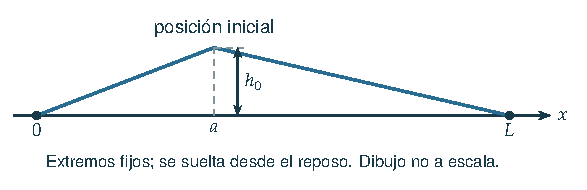
\includegraphics[width=11.13cm]{assets/M2-E0106-setup.pdf}\par
\smallskip{\small Forma inicial de la cuerda; el dibujo no está a escala.\par}
\end{minipage}
\end{center}
